\section{Modelo tomográfico y geometría}

En un modelo bidimensional idealizado de tomografía computarizada, una sección del objeto se representa mediante un coeficiente de atenuación
\[
f:\mathbb R^2\to\mathbb R,
\]
no negativo, suficientemente regular y con soporte acotado. Esta función describe la atenuación local que experimenta un haz de rayos X al atravesar el objeto.

La relación física básica entre atenuación y medición se expresa mediante la ley de Beer--Lambert. Si un haz de intensidad inicial $I_0$ recorre una trayectoria $\gamma$ y se mide una intensidad final $I$, entonces, bajo un modelo ideal sin dispersión,
\[
I=I_0\exp\left(-\int_\gamma f(x)\,ds\right).
\]
Por tanto,
\[
-\log\left(\frac{I}{I_0}\right)
=
\int_\gamma f(x)\,ds.
\]
Así, después de normalizar la intensidad y tomar logaritmos, el dato medido es una integral de línea del coeficiente de atenuación. Esta idealización y su conexión con el modelo tomográfico se presentan, por ejemplo, en Kuchment \cite[Sec.~5.3.1, pp.~23--25]{kuchment2014}.

La Figura~\ref{fig:beer-lambert} resume esta etapa física: el detector no mide directamente $f$, sino una intensidad atenuada cuya normalización logarítmica produce una integral sobre la trayectoria del haz.

\begin{figure}[htbp]
\centering
\resizebox{0.86\textwidth}{!}{\shorthandoff{<>}
\begin{tikzpicture}[font=\small]
    \draw[draw=black, fill=gray!15, thick] (0,0) ellipse (1.25 and 0.85);
    \node at (0,0.18) {objeto};
    \node at (0,-0.23) {$f(x)$};

    \draw[fill=black!10, draw=black, thick] (-4,0.55) -- (-3.35,0.9) -- (-3.35,0.2) -- cycle;
    \draw[fill=black!35, draw=black] (-4.25,0.42) rectangle (-4,0.68);
    \node[above] at (-3.75,0.92) {fuente};

    \draw[thick] (3.45,-1.45) -- (3.45,1.45);
    \foreach \y in {-1.25,-0.85,...,1.15} {
        \draw[thin] (3.35,\y) -- (3.55,\y);
    }
    \node[right] at (3.55,0) {detector};

    \draw[densely dashed, thin, gray] (-3.25,0.55) -- (3.35,1.15);
    \draw[densely dashed, thin, gray] (-3.25,0.55) -- (3.35,-0.35);
    \draw[->, thick] (-3.25,0.55) -- (3.35,0.55) node[pos=0.20, above] {$I_0$} node[pos=0.86, above] {$I$};
    \node[above] at (0,0.62) {trayectoria $\gamma$};

    \node[align=center, below] at (0,-1.45)
    {$-\log\!\left(\dfrac{I}{I_0}\right)=\displaystyle\int_\gamma f(x)\,ds$};
\end{tikzpicture}
\shorthandon{<>}
}
\caption{Adquisición tomográfica ideal y ley de Beer--Lambert. Elaboración propia.}
\label{fig:beer-lambert}
\end{figure}

En geometría paralela, las trayectorias se modelan por rectas. Para cada $\theta\in[0,\pi)$ se fija
\[
\omega(\theta)=(\cos\theta,\sin\theta),
\qquad
\omega^\perp(\theta)=(-\sin\theta,\cos\theta).
\]
En esta tesis, $\omega(\theta)$ es la normal unitaria a la recta y $\omega^\perp(\theta)$ es la dirección de integración sobre ella. Para $t\in\mathbb R$ se define
\[
L(t,\theta)
=
\{x\in\mathbb R^2: x\cdot\omega(\theta)=t\}.
\]
Equivalentemente,
\[
x=t\omega(\theta)+s\omega^\perp(\theta),
\qquad s\in\mathbb R.
\]
El parámetro $t$ es la distancia firmada de la recta al origen. Esta será la parametrización normal usada en todo el capítulo; formulaciones equivalentes pueden encontrarse en Kuchment \cite[Sec.~5.3.4, pp.~27--28]{kuchment2014}.

La Figura~\ref{fig:radon-geometria} muestra la convención geométrica usada en esta tesis: $\omega(\theta)$ es la normal de la recta y $\omega^\perp(\theta)$ es la dirección de integración.

\begin{figure}[htbp]
\centering
\resizebox{0.72\textwidth}{!}{\shorthandoff{<>}
\begin{tikzpicture}[font=\small]
    \coordinate (O) at (0,0);
    \def\ang{38}
    \def\dist{1.05}
    \coordinate (P) at (\ang:\dist);

    \draw[->, thin, gray] (-2.2,0) -- (2.3,0) node[right] {$x_1$};
    \draw[->, thin, gray] (0,-1.75) -- (0,1.9) node[above] {$x_2$};

    \draw[->, thick] (O) -- (\ang:1.65) node[above right] {$\omega(\theta)$};
    \draw[->, thin] (0.45,0) arc (0:\ang:0.45);
    \node at (0.62,0.22) {$\theta$};

    \draw[thick, black] (P) ++(\ang+90:1.45) -- ++(\ang-90:2.90) node[pos=0.86, below right] {$L(t,\theta)$};

    \draw[->, thick] (P) -- ++(\ang+90:0.95);
    \node[anchor=south east, fill=white, inner sep=1pt] at ($(P)+(\ang+90:0.78)+(-0.18,0.08)$) {$\omega^\perp(\theta)$};
    \draw[thick] (O) -- (P) node[midway, above left] {$t$};
    \fill (O) circle (1.2pt) node[below left] {$0$};
    \fill (P) circle (1.2pt);

    \draw[thin] (P) ++(\ang+90:0.18) -- ++(\ang+180:0.18) -- ++(\ang-90:0.18);
    \node[align=center] at (0,-1.45)
    {$x=t\omega(\theta)+s\omega^\perp(\theta)$,\quad $\theta\in[0,\pi)$};
\end{tikzpicture}
\shorthandon{<>}
}
\caption{Parametrización normal de las rectas en la transformada de Radon. Elaboración propia.}
\label{fig:radon-geometria}
\end{figure}

Para cada ángulo $\theta$, la función de $t$ que contiene las integrales de línea se denomina proyección. Al reunir las proyecciones para distintos valores de $\theta$ se obtiene el sinograma, es decir, la representación de los datos tomográficos en el plano de parámetros $(t,\theta)$ \cite[Sec.~5.3.5, p.~28]{kuchment2014}.

El marco físico anterior motiva el operador que se introduce en la siguiente sección. Para las demostraciones matemáticas se trabajará inicialmente con funciones $f\in\mathcal S(\mathbb R^2)$, lo cual separa el modelo físico ideal de las hipótesis analíticas usadas para justificar las identidades integrales.
